\subsection{Detection}

%\captionsetup[figure]{labelformat=empty}% redefines the caption setup of the figures environment in the beamer class.


\begin{figure}[b!]
    \centering
        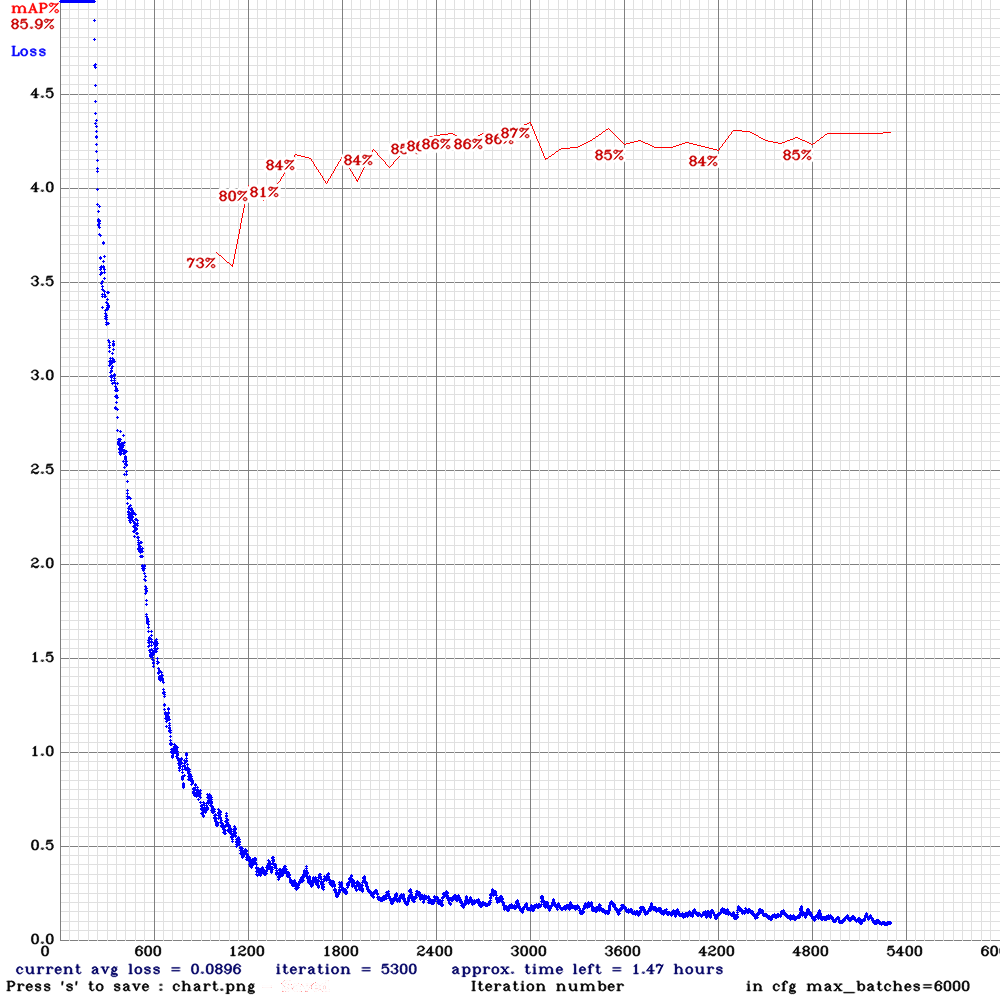
\includegraphics[width=0.4\textwidth]{pictures/painting_detection/training-v3.png}
    \caption{YOLOv3 trained on our custom dataset}
    \label{fig:training-v3}
\end{figure}

\begin{figure}[h!]
    \centering
        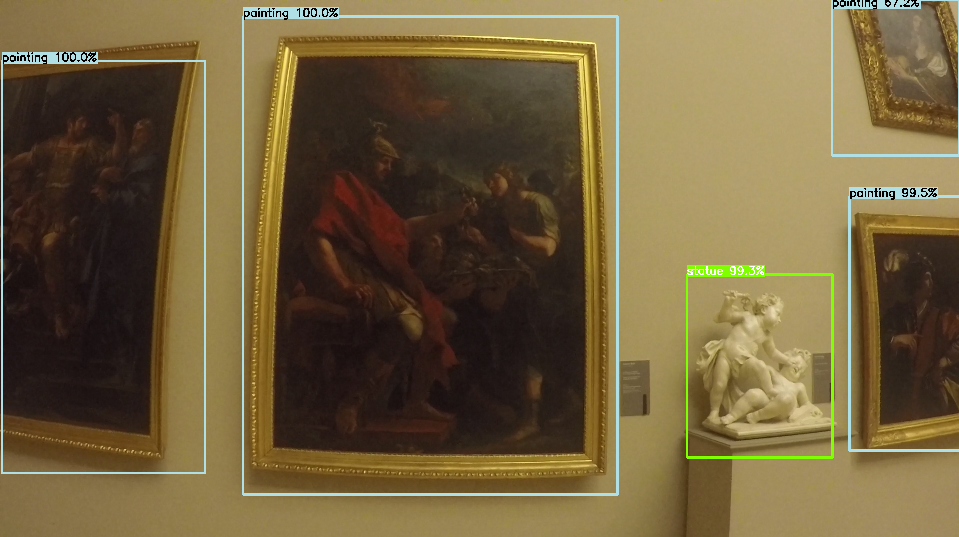
\includegraphics[width=0.45\textwidth]{pictures/painting_detection/yolo-detection2.PNG}
    \caption{Detection with YOLOv3}
    \label{fig:yolo_detection}
\end{figure}



\begin{figure*}[h]
    \minipage{0.45\textwidth}
      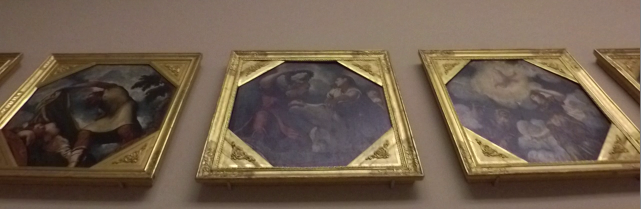
\includegraphics[width=\linewidth]{pictures/painting_detection/shadow1.PNG}
      \caption*{Image with shadow}\label{fig:shadow1}
    \endminipage\hfill
    \minipage{0.45\textwidth}
      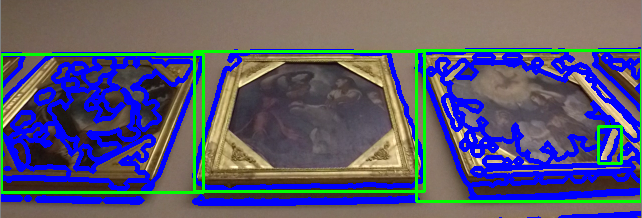
\includegraphics[width=\linewidth]{pictures/painting_detection/shadow2.PNG}
      \caption*{Not precise bounding box}\label{fig:shadow2}
    \endminipage\hfill
    \caption{Inaccurate detection due to the shadows}\label{fig:innaccurate_detection}
\end{figure*}







The detection of paintings, statues and person is done through a custom YOLOv3 neural network~\cite{yolov3}.
Yolo is an architecture that provides a new approach to object detection, a single neural network predicts bounding boxes and class probabilities directly from full images in one evaluation.
In order to use this neural network we have labeled 1343 images, 805 of them have been used to train the network, 269 for the validation set and 269 for the test set, providing a total number of 3733 labels. The images of paintings and statues were taken from frames extracted by some videos recorded in the Galleria Estense, for the person class was instead used a mix of images taken from the previous videos and some images of people in another museum to increase generalization.
The training has been performed with darknet~\cite{darknet} taking the mAP every 1000 iterations (fig.~\ref{fig:training-v3}), this allowed us to take the best weights that weren't affected by overfitting.
In the end we got a powerful neural network with high performance (fig.~\ref{fig:yolo_detection}) and capable of a good generalization (tab.~\ref{tab:detection_performance}).
An important point is the data management: the train set, the validation set and the test set have been balanced, this allowed the network to have a better performance and predict classes in a correct way.



\begin{table*}[ht!]
    \centering
\begin{tabular}{|c|c|c|c|c|}
\hline
\multicolumn{5}{|c|}{\textbf{Detection Performance}}       \\ \hline
\multicolumn{1}{|l|}{} & \textbf{Painting} & \textbf{Statue} & \textbf{Person} & \textbf{Overall} \\ \hline
\textbf{TP}        & 550     & 174     & 125     & 849     \\ \hline
\textbf{FP}        & 107     & 19      & 32      & 158     \\ \hline
\textbf{Precision} & 83,71\% & 90,16\% & 79,62\% & 84,31\% \\ \hline
\textbf{Recall}    & -       & -       & -       & 94\%    \\ \hline
\textbf{Average IoU}       & -       & -       & -       & 71\%    \\ \hline
\textbf{AP}        & 97,29\% & 98,61\% & 75,45\% & -       \\ \hline
\textbf{mAP}       & -       & -       & -       & 90,45\% \\ \hline
\end{tabular}
\caption{Detection Performance with YOLOv3}
    \label{tab:detection_performance}
\end{table*}



\subsubsection{Comparison with previous technique}
In a previous pipeline (fig.~\ref{fig:pipeline_detection}) the detection was made without neural networks: the image was at first transformed in a gray level image, preprocessed with adaptive threshold, median blur \cite{median-blur} to remove the noise and opening, and then compute the borders.
After the preprocessing, the pipeline uses the result to compute the  Connected Component Labeling~\cite{Grana_ccl} to label the background and the foreground objects.
In order to label the foreground objects as paintings, the components needed to have an entropy grater than a threshold, and then the bounding boxes were drawn.
Despite this method worked well in some scenerios, it wasn't able to adapt to strong luminance variation, to manage the presence of shadows (fig~\ref{fig:innaccurate_detection}) and to generalize with all the classes. Many times the shadow was recognized as an object or as part of the painting and for this reason the IoU was computed with not optimal performance, this reason led us to choose to implement a neural network.

